\documentclass{beamer}
\usepackage[italian]{babel}

\DeclareMathOperator{\lcm}{lcm}

\title{Presentazione PHPC}
\author{Pierluigi Supino \and Rodolfo Diana \and Salvatore Di Gennaro}

\usetheme{default}
\begin{document}
\begin{frame}
    \titlepage
\end{frame}

\begin{frame}{Implementazione}
    In ambiente multi-nodo e multi-GPU, il prodotto tra matrici viene scomposto in due sottoproblemi:
    \begin{enumerate}
        \item gestione a livello globale tra i processi, ovvero come suddividere le matrici e quali comunicazioni eseguire;
        \item gestione a livello locale all'interno di ciascun nodo, ovvero come eseguire il prodotto sfruttando le GPU a disposizione.
    \end{enumerate}
\end{frame}

\begin{frame}{Implementazione}{Processi}
    \begin{itemize}
        \item Scalable Universal Matrix Multiplication Algorithm (SUMMA)
        \item Algoritmo efficiente e scalabile per ogni numero di processi
    \end{itemize}
\end{frame}

\begin{frame}{Implementazione}{Processi - SUMMA}
    \begin{itemize}
        \item Si dispongono i processi in una griglia $r \times c$
    \end{itemize}
    \begin{figure}
        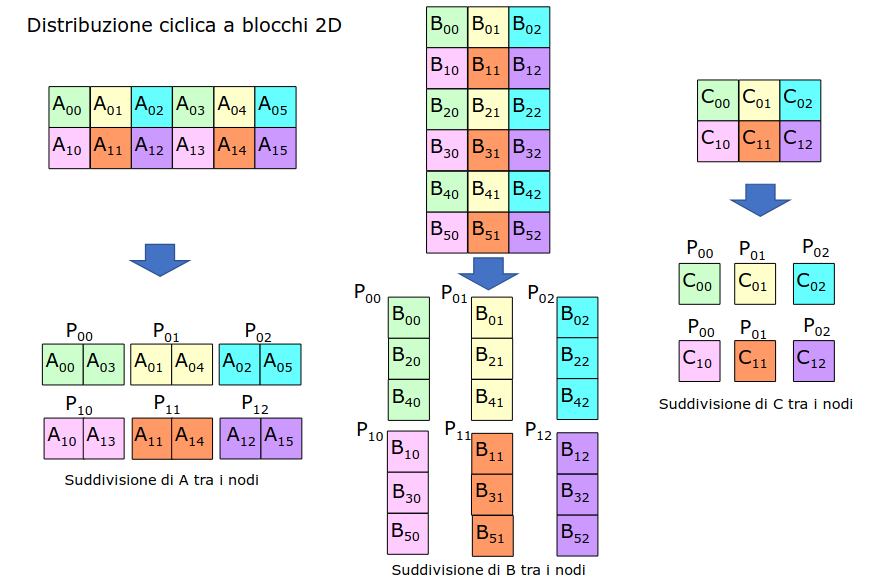
\includegraphics[width=0.5\linewidth]{imgs/summa.png}
        \caption{Distribuzione SUMMA}
    \end{figure}
\end{frame}

\begin{frame}{Implementazione}{Processi - SUMMA}
    Semplificazioni e assunzioni effettuate:
    \begin{itemize}
        \item solo matrici quadrate $n \times n$, con $n$ multiplo di $\lcm(r,c)$
        \item matrici di input di ogni processo come array contigui \textit{row-major} contenenti già i dati necessari
        \item gestione degli errori quasi assente per evitare overhead
    \end{itemize}
\end{frame}

\begin{frame}{Implementazione}{MultiGPU}
    \begin{itemize}
        \item Più GPU per processo: come suddividere il lavoro?
              \begin{itemize}
                  \item Vogliamo eseguire le operazioni in parallelo
                        \begin{enumerate}
                            \item Evitare conflitti di memoria da serializzare
                            \item Nessuna funzione bloccante per l'host
                        \end{enumerate}
              \end{itemize}
        \item Possibili soluzioni:
              \begin{itemize}
                  \item Pattern fork-join con ogni thread che gestisce una GPU
                  \item \alert{Utilizzo dei metodi async e degli stream di CUDA}
              \end{itemize}
    \end{itemize}
\end{frame}


\begin{frame}{Implementazione}{MultiGPU - CUDA}
    \begin{itemize}
        \item CUDA stream: code di operazioni da gestire in sequenza
              \begin{itemize}
                  \item Operazioni in stream diversi potrebbero essere eseguite in concorrenza
                  \item Operazioni in stream diversi potrebbero essere alternate
                  \item Se non viene specificato uno stream viene usato lo stream 0 (bloccante)
              \end{itemize}
        \item I trasferimenti sono davvero asincroni solo se la memoria indirizzata è \textit{page-locked}
              \begin{itemize}
                  \item cudaMallocHost
                  \item cudaHostRegister/cudaHostUnregister
              \end{itemize}
    \end{itemize}
\end{frame}

\begin{frame}{Implementazione}{MultiGPU - cuBLAS}
    \begin{itemize}
        \item Problema del prodotto matriciale già ampiamente discusso
        \item Numerose librerie disponibili: \alert{cuBLAS}
              \begin{itemize}
                  \item implementazione ottimizzata per GPU NVIDIA delle specifiche BLAS
                        \begin{itemize}
                            \item Per compatibilità con Fortran si aspetta ordine column-major
                            \item Basta calcolare $\mathbf{C}^T=(\mathbf{B}\mathbf{A})^T$
                        \end{itemize}
                  \item \alert{cuBLASXt}: estensione per ambienti multi-GPU
              \end{itemize}
    \end{itemize}
\end{frame}


\end{document}